\section{Zero-Shot Rewards from Human Videos}
\label{sec:method_reward}

We aim to learn a multi-task reward function by learning from human demonstrations. For each task $\mathcal{T}_i$, the reward function $\mathcal{R}$ will be conditioned on one of $K$ human demonstrations $\mathcal{D}_i = \{ d_{i,j} \}_{j=1}^K$ specifying the desired task. 

Then, given the robot environment's state space $\mathcal{S}^r$, action space of the robot $\mathcal{A}^r$, and robot dynamics $f^r(s' | s, a)$, we want to solve the MDP parameterized by $(\mathcal{S}^r, \mathcal{A}^r, f^r, \mathcal{R})$ for a task $\mathcal{T}_i$.

\begin{figure}[H]
\centering
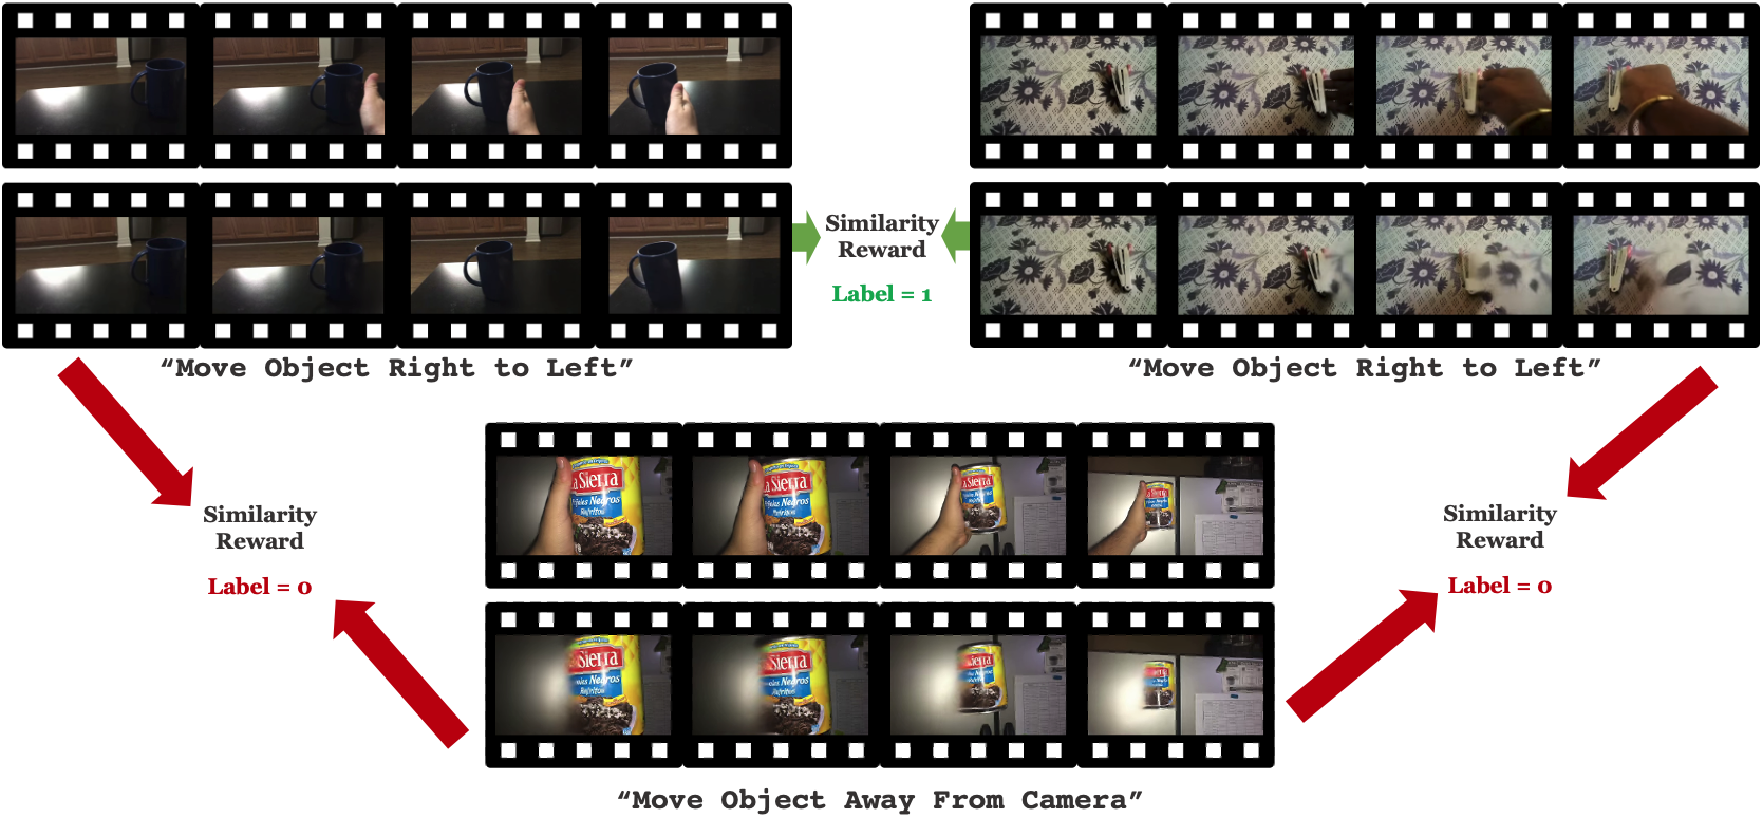
\includegraphics[width=\linewidth]{figs_reward/method_overview.pdf}
\vspace{-0.2in}
   \caption{\small Training Overview: Human data is processed as follows. We generate masks for human arms and hands in videos from the Something-Something dataset \cite{smthsmth}. Videos that do not have high-quality masks are discarded. The remaining videos are inpainted based on their masks. We take this set of inpainted human videos and learn a discriminator to capture the functional features of the video.}
    \label{fig:method_reward}
    \vspace{-0.15in}
\end{figure}

\subsection{Learning Agent-Agnostic Representations}

Our work addresses the embodiment gap by visually removing the agent from the scene at both training and test time. There are a few potential inpainting methods we can use when given masks to remove the agent (human or robot) from a video. To generate the masks for the robot arm, we used Detectron2 \cite{detectron2}, a state-of-the-art segmentation method, and fine-tuned it for detecting our robot. However, we found Detectron2 to be unreliable in detecting human hands and arms in egocentric data. We believe this is because Detectron2 was trained on third-person views of humans where most of the body is in the scene. For masking human hands and arms in human videos, we use EgoHOS \cite{egohos}, a method trained on egocentric videos from datasets like Ego4D \cite{ego4d} and Epic-Kitchens \cite{epickitchens}. 

While this method provides more consistent masks, there are still videos that have few or noisy masks due to occlusion or difficult lighting conditions. We refine our dataset by removing videos where fewer than half of the frames have human masks. This removes only one-fifth of our dataset, so we still keep a large majority of our data for training.

For inpainting, we considered two types of methods. We can utilize a video inpainting method such as Copy and Paste Networks \cite{cpnetworks} or E2FGVI \cite{e2fgvi}. Another option for inpainting is to inpaint frame-by-frame, such as with Stable Diffusion \cite{stablediffusion}. We found that video inpainting methods perform better as they have access to context for occlusions that singular images do not have. Stable Diffusion also requires many denoising iterations that reduce its speed.

\subsection{Addressing Visual Domain Gap}

While training on a large dataset with a variety of objects, lighting, and poses will provide some generalization, we conjecture that it might not be sufficient to generalize to simulation environments, which look significantly different from the real world. As a result, we account for the visual differences between simulation and real-world settings. In particular, we use Stable Diffusion \cite{stablediffusion}, a pre-trained image-text generative model, to create synthetic videos by augmenting existing videos from the dataset.

To augment a video, we take individual frames from the video and generate a novel set of frames. We guide this image-to-image translation using text conditioning. That is, given a text prompt $T$ and video $V$, for each frame $ v_1, v_2, \dots, v_n \in V$ we use Stable Diffusion as a function $g$ to map it to new frame $v'_i = g(v_i, T)$. In order to promote generalization to simulation environments, we use prompts $T$ such as \verb|"OpenGL style rendering"|, and \verb|"Unity style rendering"| to to encourage the output frames to match the desired style.

Because this approach generates a video by transforming individual frames, this does not necessarily maintain the temporal consistency of the video. In order to keep the videos coherent, we restrict the noise added to individual frames to be sampled within a reasonable range for each video.

\subsection{Reward Training}
The reward function we want to learn is $\mathcal{R} (s_{1:T}, \mathcal{D}_i)$. Here, for each task $\mathcal{T}_i$, we have a set of human demonstrations $\mathcal{D}_i$.

We will use a pretrained inpainting method $\phi^h$ for human inpainting and $\phi^r$ for robot inpainting. During training, we can apply $\phi^h$ to each demonstration and train the DVD encoder $f_{\text{enc}}$ and similarity function $f_{\text{sim}}$ as described in their paper \cite{DVD}.

To summarize the training method in DVD, we train $\mathcal{R}$ as follows. We use a pretrained encoder $f_{\text{enc}}$ and a learned similarity function $f_{\text{sim}}$ to generate the pairwise reward:

\vspace{-0.3cm}

$$\mathcal{R}(d_i, d_j) = f_{\text{sim}}(f_{\text{enc}}(\phi^h(d_i)), f_{\text{enc}}(\phi^h(d_j))).$$

When learning $\mathcal{R}$ at training time, note that $f_{\text{enc}}$ and $\phi^h$ are pretrained and frozen. To learn $f_{\text{sim}}$, we sample videos $d_i^1, d_i^2, d_j \in \mathcal{D}$. We minimize the cross-entropy loss below:

\vspace{-0.3cm}

$$\mathcal{L} = \mathbb{E}_{(d_i^1, d_i^2, d_j) \sim \mathcal{D}} [\log (\mathcal{R}(d_i^1, d_i^2)) + \log (1 - \mathcal{R}(d_i^1, d_j)]$$

Note that this is essentially contrastive loss over demonstrations from different tasks. Above, $d_i^1$ is the anchor, $d_i^2$ is a positive sample and $d_j$ is the negative sample.

\subsection{Task Execution}

\begin{figure}[H]
\centering
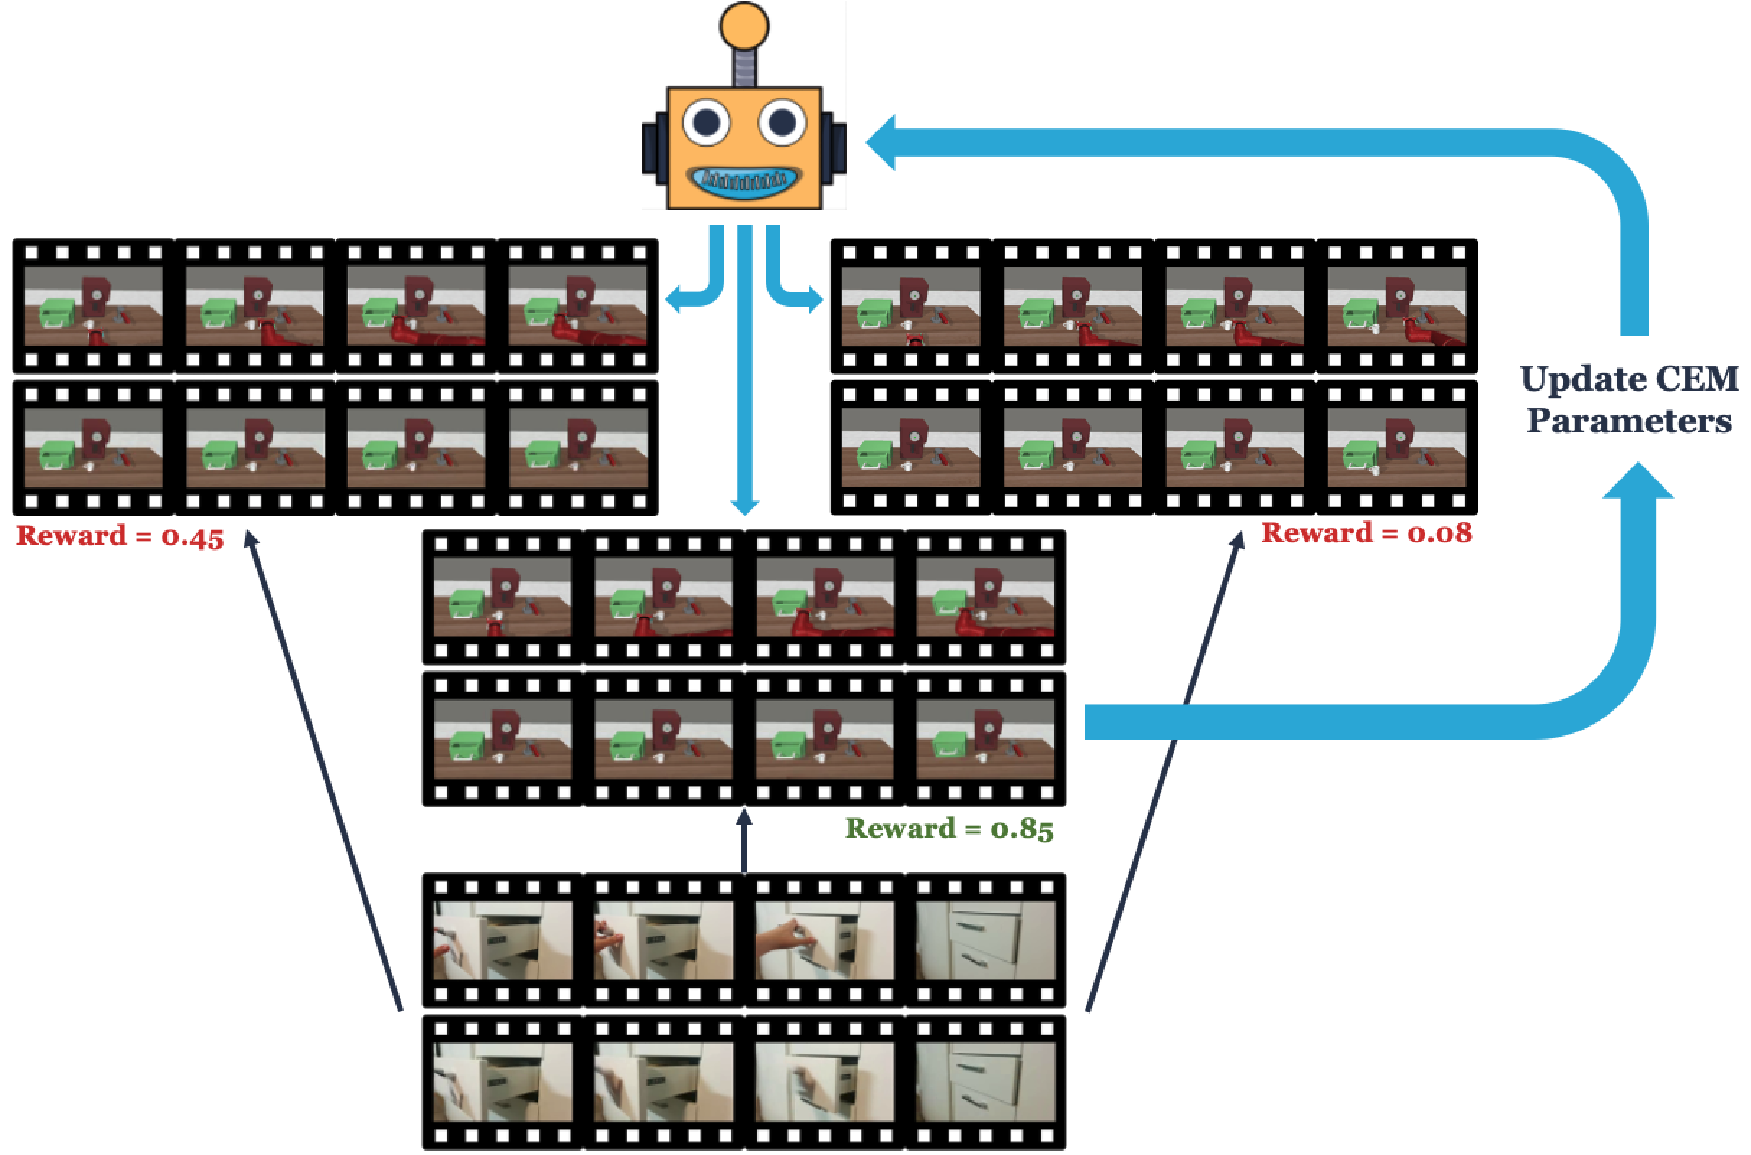
\includegraphics[width=\linewidth]{figs_reward/method_optimization.pdf}
\vspace{-0.2in}
   \caption{\small At test time, we take as input a set of human demonstrations of the same task. Using trajectories sampled from CEM, we use our reward function to judge the similarity between every (demo, trajectory) pair. We use CEM to optimize this reward function to generate trajectories that are most functionally similar to the demos.}
    \label{fig:method_test}
    \vspace{-0.15in}
\end{figure}

At test time, we are given a set of human demonstrations $\mathcal{D}_i = \{ d_{i,j} \}_{j=1}^K$ for a specific task. We have a reward function $\mathcal{R}$ that can take in a robot trajectory $s_{1:T}$ and a single human demonstration $d_{i, j}$. We calculate the reward with the corresponding inpainting function, as follows:

$$\mathcal{R}(s_{1:T}, d_{i, j}) = f_{\text{sim}}(f_{\text{enc}}(\phi^r(s_{1:T})), f_{\text{enc}}(\phi^h(d_{i, j})))$$

We can optimize for this reward function using zeroth order methods like Cross-Entropy Method (CEM) or Model Predictive Path Integral (MPPI) control. For our method, we implement CEM. CEM keeps track of a trajectory distribution parameterized by a Gaussian for each action $a_i \sim \mathcal{N}(\mu_i, \sigma_i)$ for $i = 1 \dots T$. CEM then takes multiple samples from this distribution and retains the samples (elites) with the largest rewards to update the distribution for the next iteration. Then from this distribution, CEM rolls out a trajectory to act out an episode.

For the results in Table~\ref{table:baseline_comparison_reward}, we use the ground truth dynamics from the simulator when rolling out samples taken from the action distribution. We can also potentially use a state or visual dynamics function such as \cite{hafner2019dreamer} learned in the environment to run CEM efficiently in a closed-loop fashion.


\subsection{Datasets and Environments}

We generate results in Metaworld \cite{metaworld}, with a tabletop environment that has a mug, drawer, and faucet. We train our models using the Something-Something dataset \cite{smthsmth}, an egocentric dataset of humans manipulating different objects according to various tasks. We primarily evaluate our method on three tasks: \textit{Close Drawer}, \textit{Push Mug Away}, and \textit{Move Mug Right}. We train on a dataset of around 10K videos which are labeled with task information. This dataset consists of data for 6 tasks, of which three are the evaluation tasks specified above.